\documentclass{article}

\usepackage[margin=1in]{geometry}
\usepackage{amsmath}
\usepackage{graphicx}
\usepackage{subfig}

\author{Damien Prieur}
\title{Assignment 3 \\ CS 435}
\date{}

\begin{document}

\maketitle

\section{Theory Questions}
\begin{enumerate}
\item If the matrix below is the energy of image
$$
\begin{bmatrix}
2&	3&	4&	5&	1\\
1&	0&	2&	2&	1\\
4&	3&	5&	1&	2\\
4&	4&	4&	4&	6\\
4&	5&	2&	0&	2\\
2&	3&	3&	0&	3\\
\end{bmatrix}
$$

\begin{enumerate}
\item Construct the optimal seam matrix if we assume vertical seams
$$
\begin{bmatrix}
2&	3&	4&	5&	1\\
3&	2&	5&	3&	2\\
6&	5&	7&	3&	4\\
9&	9&	7&	7&	9\\
13&	12&	9&	7&	9\\
14&	12&	10&	7&	10\\
\end{bmatrix}
$$
\item What is the optimal seam?
$$
\begin{bmatrix}
2&	3&	4&	5&	X\\
3&	2&	5&	2&	X\\
6&	5&	7&	X&	2\\
9&	9&	7&	X&	9\\
13&	12&	9&	X&	9\\
14&	12&	10&	X&	10\\
\end{bmatrix}
$$
\end{enumerate}
\end{enumerate}

\newpage
\section{Image Resizing}
First grab two images of interest to you so that we can multiple example I/O of each approach.   Next allow a user (either via prompt, parameter passing, or changing variable values) to provide a desired height and width.\\ 

\noindent
We'll refer to the original height and width as $h$ and $w$, respectively, and the new height and width as $h\prime$ and $h\prime$, respectively.  Do this all in color!  You may \textbf{not} use any Matlab functions (for instance, \emph{imresize}) to do these changes for you.\\   

\noindent
Implement the following resizing techniques:
\begin{itemize}
\item Do nearest neighbor sampling.   Go through each location in your new target image, $(x\prime, y\prime)$, and assign it the value of the nearest pixel, whose location is $(x, y) = round(x\prime \frac{w}{w\prime}, y\prime \frac{h}{h\prime})$.
\item Do linear interpolation.   Go through each location in your new target image, $(x\prime, y\prime)$, and compute the \emph{ideal} floating point location as $(x, y) =(x\prime \frac{w}{w\prime}, y\prime \frac{h}{h\prime})$.  Compute the values for location $(x\prime, y\prime)$ by linearly interpolating the values of the four pixels nearest $(x,y)$ (using Euclidean distance).
\end{itemize}

\noindent
For your report provide sample I/O for both your test images, using both of these techniques, for two different values of $(w\prime, h\prime)$ (8 total images).

\newpage
\begin{figure}[h!]
    \centering
    \subfloat[Img 1 original]{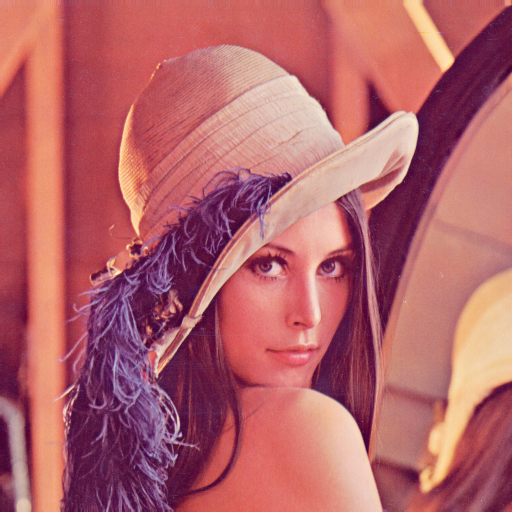
\includegraphics[scale=.2]{images/Lenna.png}}
    \\
    \subfloat[Img 1 Nearest Neighbor 1]{\includegraphics[scale=.2]{images/generated/Q2_img_1_nearest_1.png}}
    \qquad
    \subfloat[Img 1 Linear Interpolation 1]{\includegraphics[scale=.2]{images/generated/Q2_img_1_linear_1.png}}
    \\
    \subfloat[Img 1 Nearest Neighbor 2]{\includegraphics[scale=.2]{images/generated/Q2_img_1_nearest_2.png}}
    \qquad
    \subfloat[Img 1 Linear Interpolation 2]{\includegraphics[scale=.2]{images/generated/Q2_img_1_linear_2.png}}
\end{figure}
\newpage

\begin{figure}[h!]
    \centering
    \subfloat[Img 2 original]{\includegraphics[scale=.2]{images/aloeR.jpg}}
    \\
    \subfloat[Img 2 Nearest Neighbor 1]{\includegraphics[scale=.2]{images/generated/Q2_img_2_nearest_1.png}}
    \qquad
    \subfloat[Img 2 Linear Interpolation 1]{\includegraphics[scale=.2]{images/generated/Q2_img_2_linear_1.png}}
    \\
    \subfloat[Img 2 Nearest Neighbor 2]{\includegraphics[scale=.2]{images/generated/Q2_img_2_nearest_2.png}}
    \qquad
    \subfloat[Img 2 Linear Interpolation 2]{\includegraphics[scale=.2]{images/generated/Q2_img_2_linear_2.png}}
\end{figure}
\newpage

\section{Energy Function}
We're also going to want to explore seam carving.  The first part of that requires computing the energy functions of your images.\\

\noindent
For each of your images, compute its energy and visualize this as an image.\\

\noindent
Some implementation details:
\begin{itemize}
\item Do this in grayscale
\item First smooth your grayscale image using a Guassian filter prior to getting the gradients (or do this in one step).  Choose parameters that make sense for you (and report them!).  \textbf{You must} provide your own smoothing and gradient kernels.
\item Pad your images such that the convolution processes don’t change the size of the image.
\item Since you already demonstrated in HW1 your ability to implement RGB to Gray and convolution, for this assignment \textbf{may} use Matlab functions like $conv2, rgb2gray$.
\end{itemize}

\begin{figure}[h!]
    \centering
    \subfloat[Image 1 energy]{\includegraphics[scale=.4]{images/generated/Q3_img_1_energy.png}}
    \subfloat[Image 2 energy]{\includegraphics[scale=.2]{images/generated/Q3_img_2_energy.png}}
\end{figure}

\newpage

\section{Optimal Seam}
Now that you have your energy images, we must find the optimal seam in it.\\

\noindent
Using the technique discussed in class, for each of your images, 

\begin{itemize}
\item Use its energy image to compute a seam matrix.
\item Find the optimal seam in this seam matrix via backtracing.
\item Superimpose on your color image the optimal seam in red.
\end{itemize}

\noindent
Additional Details:
\begin{itemize}
\item We will do vertical seam carving, starting at the top of the image.
\item You’ll likely have to think about how to handle the edge cases.
\end{itemize}

\noindent

\begin{figure}[h!]
    \centering
    \subfloat[Image 1 Optimal Seam]{\includegraphics[scale=.4]{images/generated/Q4_img_1_highlighted_seam.png}}
    \subfloat[Image 2 Optimal Seam]{\includegraphics[scale=.2]{images/generated/Q4_img_2_highlighted_seam.png}}
\end{figure}

\newpage

\section{Seam Carving}
Finally, let's use seam carving to reduce the aspect ratio. Since we found the optimal \emph{vertical} seam in the previous part, we'll just reduce the width, from it's original width down to one pixel wide. \\

\noindent
For each of your images, create a video showing the seam removal process.  Each frame of the video should depict the current color image with the current optimal seam superimposed (like in the previous part). \\

\noindent
Note:
\begin{itemize}
\item You may need to “pad” your frames so that they all have the same size in order to render as a movie.
\item To create a movie in Matlab use the \emph{VideoWriter} class.  In addition, to keep the movies relatively small in file size, use the \emph{MPEG-4} profile for your VideoWriter object.
\end{itemize}

\newpage

\end{document}
